\documentclass[11pt,a4paper]{ctexart}
\usepackage[utf8]{inputenc}
\usepackage{geometry}
\geometry{left=2.5cm,right=2.5cm,top=2.8cm,bottom=2.8cm}
\usepackage{amsmath,amssymb,amsfonts}
\usepackage{enumitem}
\usepackage{titlesec}
\usepackage{xcolor}
\usepackage{tcolorbox}
\usepackage{hyperref}

% 引入绝对位置放置宏包用于生成水印及插入图片宏包
\usepackage{graphicx}
\usepackage{eso-pic}



% --- 颜色定义 ---
\definecolor{mainblue}{RGB}{26, 82, 118}
\definecolor{secblue}{RGB}{41, 128, 185}
\definecolor{bglight}{RGB}{244, 246, 247}
\definecolor{textdark}{RGB}{44, 62, 80}

% --- 页面美化与字体设置 ---
\hypersetup{colorlinks=true, linkcolor=mainblue, urlcolor=secblue}
\setlist[itemize]{leftmargin=2em, itemsep=0.3em}
\setlist[enumerate]{leftmargin=2em, itemsep=0.3em}

% --- 标题样式自定义 ---
\titleformat{\section}{\large\bfseries\color{mainblue}}{\thesection}{1em}{}[{\color{mainblue}\titlerule[1pt]}]
\titleformat{\subsection}{\normalsize\bfseries\color{secblue}}{\thesubsection}{1em}{}
\titleformat{\subsubsection}{\small\bfseries\color{textdark}}{\thesubsubsection}{1em}{}

% --- 水印设置 (每页三个，斜45度，居中分布) ---
\newcommand{\WMText}{贺昱琪学习资料}
\newcommand{\WMScale}{2.28}
\newcommand{\WMAngle}{45}
\colorlet{WMColor}{black!8}

\AddToShipoutPictureBG{%
  \AtPageLowerLeft{%
    \put(\LenToUnit{0.66\paperwidth},\LenToUnit{0.70\paperheight}){%
      \rotatebox{\WMAngle}{\scalebox{\WMScale}{\textcolor{WMColor}{\WMText}}}%
    }%
    \put(\LenToUnit{0.33\paperwidth},\LenToUnit{0.50\paperheight}){%
      \rotatebox{\WMAngle}{\scalebox{\WMScale}{\textcolor{WMColor}{\WMText}}}%
    }%
    \put(\LenToUnit{0.66\paperwidth},\LenToUnit{0.30\paperheight}){%
      \rotatebox{\WMAngle}{\scalebox{\WMScale}{\textcolor{WMColor}{\WMText}}}%
    }%
  }%
}

\begin{document}

\begin{center}
    \LARGE \textbf{贺昱琪专项训练五}
\end{center}

\vspace{0.5cm}

\noindent \textbf{一、细心算一算}

\begin{enumerate}
    \item[1.] 计算（每小题 5 分，共 20 分）
    \begin{enumerate}
        \item[(1)] $2\frac{3}{5} \times \frac{3}{4} - \frac{2}{5} \times \frac{3}{4}$
        \vspace{3.5cm}
        
        \item[(2)] $3.64 \times \frac{1}{4} + 4.36 \times 0.25$
        \vspace{3.5cm}
        
        \item[(3)] $\left[ 7\frac{1}{2} - \left( 1\frac{5}{8} - \frac{1}{2} \times \frac{3}{4} \right) \right] \div 3$
        \vspace{3.5cm}
        
        \item[(4)] $\left[ \frac{8}{9} \times \left( \frac{4}{5} - 0.35 \right) + 30\% \right] \div \frac{3}{5}$
        \vspace{3.5cm}
    \end{enumerate}
    
    \item[2.] 解方程（每小题 5 分，共 10 分）
    \begin{enumerate}
        \item[(1)] $\frac{2}{3}x - 1 = \frac{1}{2}x$
        \vspace{3.5cm}
        
        \item[(2)] $\frac{x-2}{0.5} - \frac{x+1}{3} = 2$
        \vspace{3.5cm}
    \end{enumerate}
\end{enumerate}

\vspace{0.8cm}

\noindent \textbf{二、用心想一想}

\begin{enumerate}
    \item[3.] (10分) 如图是一幢大楼的两个接雨器（箭头处为大小相同的接雨孔），雨水将图 1 接雨器注满需要 2 小时，那么将图 2 接雨器注满需要多少小时？
    \begin{center}
        
\includegraphics[width=0.5\textwidth]{3.png}
    \end{center}
    \vspace{4.0cm}
    
    \item[4.] (10分) A、B 两地之间是山路，相距 240 千米，其中一部分是上坡路，其余是下坡路。某人骑电动车从 A 地到 B 地，再沿原路返回，去时用了 11 小时，返回时用了 9 小时。已知下坡路每小时行驶 30 千米，那么上坡路每小时行驶多少千米？
    \vspace{4.5cm}
\end{enumerate}

\vspace{0.8cm}

\noindent \textbf{三、认真填一填（每小题 4 分，共 40 分）}

\begin{enumerate}
    \item[5.] 
    \begin{minipage}{0.65\textwidth}
        下列选项中，通过旋转左侧图案，无法得到的是\underline{\hspace{2cm}}。
    \end{minipage}
    \hfill
    \begin{minipage}{0.3\textwidth}
        \centering
        
\includegraphics[width=\linewidth]{5.png}
    \end{minipage}
    \vspace{1.2cm}
    
    \item[6.] 字母 A、B、C 按一定的规律排列：ABBCCCABBCCCABBCCC... 第 2024 个字母是\underline{\hspace{2cm}}。\vspace{1.2cm}
    
    \item[7.] 
    \begin{minipage}{0.65\textwidth}
        如图，阴影部分的周长是\underline{\hspace{2cm}}厘米。（结果保留 $\pi$）
    \end{minipage}
    \hfill
    \begin{minipage}{0.3\textwidth}
        \centering
        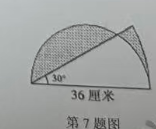
\includegraphics[width=\linewidth]{7.png}
    \end{minipage}
    \vspace{1.2cm}
    
    \item[8.] 一桶水，需 2 人一起抬。3 人轮流把一桶水从离家 450 米远的地方抬回家，平均每人要抬\underline{\hspace{2cm}}米。\vspace{1.2cm}
    
    \item[9.] 
    \begin{minipage}{0.65\textwidth}
        如图，圆柱的底面积与侧面积的比是 $1:8$。把这个圆柱沿半径切分成若干等份，拼成一个近似长方体。若近似长方体的表面积比圆柱的表面积增加了 40 平方厘米，则圆柱的底面积是\underline{\hspace{2cm}}平方厘米。（结果保留 $\pi$）
    \end{minipage}
    \hfill
    \begin{minipage}{0.3\textwidth}
        \centering
        
\includegraphics[width=\linewidth]{9.png}
    \end{minipage}
    \vspace{1.2cm}
    
    \item[10.] 红、黄两根彩带共长 52 米，红彩带剪去 25\%，黄彩带剪去 3 米，两根彩带剩下的部分一样长。原来红彩带长\underline{\hspace{2cm}}米。\vspace{1.2cm}
    
    \item[11.] 
    \begin{minipage}{0.65\textwidth}
        如图，$\triangle ABC$ 的面积是 36 平方厘米，$AD=DE=EC$，$F$ 是 $BC$ 中点，$FG=GC$，阴影部分的面积是\underline{\hspace{2cm}}平方厘米。
    \end{minipage}
    \hfill
    \begin{minipage}{0.3\textwidth}
        \centering
        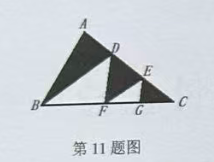
\includegraphics[width=\linewidth]{11.png}
    \end{minipage}
    \vspace{1.2cm}
    
    \item[12.] 
    \begin{minipage}{0.65\textwidth}
        如图，小军用编号 1、2、3、4、5 的大小不同的正方形拼出一个长方形，则中间 5 号正方形的边长是\underline{\hspace{2cm}}厘米。
    \end{minipage}
    \hfill
    \begin{minipage}{0.3\textwidth}
        \centering
        
\includegraphics[width=\linewidth]{12.png}
    \end{minipage}
    \vspace{1.2cm}
    
    \item[13.] 桌上放有一张写有 61 的卡片，若从桌子的另一侧看去，却是 19。现在桌子上放着这样一道算术题：$89+16+69+6\square+\square 8=88$。甲、乙两位同学面对面坐在桌子两侧，而他们计算这道数学题的结果恰好相同，则两个方格中应填的数字和是\underline{\hspace{2cm}}。\vspace{1.2cm}
    
    \item[14.] 
    \begin{minipage}{0.65\textwidth}
        如图，为一个 3 行 3 列的表格，当空格内填上适当的数后，每行、每列以及每条对角线上的数字之和都是相等的，则 $k=$\underline{\hspace{2cm}}。
    \end{minipage}
    \hfill
    \begin{minipage}{0.3\textwidth}
        \centering
        
\includegraphics[width=\linewidth]{14.png}
    \end{minipage}
\end{enumerate}

\vspace{0.8cm}

\noindent \textbf{四、勇敢闯一闯}

\begin{enumerate}
    \item[15.] (12分) 某音乐厅月初决定在暑假期间举办学生专场音乐会，入场券分为团体票和零售票，其中团体票占总票数的 $\frac{2}{3}$。若提前购票，则给予不同程度的优惠。在 5 月份内，团体票每张 12 元，共售出团体票数的 $\frac{3}{5}$；零售票每张 16 元，共售出零售票数的一半。如果在 6 月份内，团体票按每张 16 元出售，并计划 6 月份内售出全部余票，那么零售票应按每张多少元定价才能使这两个月的票款收入持平？
    \vspace{4.5cm}
    
    \item[17.] (18分) 
    \begin{enumerate}
        \item[] 【新知学习】用水平线和竖直线将平面分成若干个边长为 1 的小正方形格子，小正方形的顶点叫格点，以格点为顶点的多边形叫格点多边形。奥地利数学家皮克发现了一个计算格点多边形面积的公式：$S = a + \frac{b}{2} - 1$。其中 $a$ 表示多边形内部的格点数，$b$ 表示多边形边界上的格点数，$S$ 表示多边形的面积。\\
        若方格纸中，每个小正方形边长为 1。图 1 中四边形的面积为\underline{\hspace{2cm}}；图 2 中四边形的面积为\underline{\hspace{2cm}}。
        \item[] 【实践应用】小新同学对“皮克公式”很感兴趣，他拿出珍藏的方格纸如图 3，他希望画出面积为 4 的格点六边形，并使得方格纸上两个核心点均位于六边形的内部。请你帮助小新设计三个形状不同的符合要求的格点六边形。
    \end{enumerate}
    \begin{center}
        
\includegraphics[width=0.7\textwidth]{17.png}
    \end{center}
\end{enumerate}

\end{document}